\chapter{Trabalhos Relacionados}
\label{cap:trabalhos_relacionados}

Neste capítulo, são abordados conceitos fundamentais que regem o mercado financeiro, juntamente com a análise de trabalhos prévios focados na previsão e recomendação de compra e venda de ativos em diversos mercados. Inicialmente, na Seção \ref{subsec:series_temporais}, é apresentado o conceito de séries temporais, que posteriormente é relacionado com o mercado financeiro na Seção \ref{subsec:mercado_financeiro}. Em seguida, na Seção \ref{subsec:abordagem}, é descrita uma estrutura padrão seguida por grande parte dos trabalhos analisados. Na Seção \ref{subsec:conjunto_dados}, são apresentadas as variáveis utilizadas para a construção do conjunto de dados. A seguir, na Seção \ref{subsec:geracao_novas_variaveis}, é abordado o conceito de geração de variáveis a partir das já existentes. Na Seção \ref{subsec:selecao_variaveis}, são discutidas técnicas de seleção das variáveis mais relevantes para o problema. Na Seção \ref{subsec:tecnicas_predicao}, são apresentados modelos computacionais e matemáticos utilizados para a predição dos valores ou tendências. Posteriormente, na Seção \ref{subsec:estrategias}, são abordadas estratégias utilizadas para a tomada de decisão na bolsa. Na Seção \ref{subsec:criterio_avaliacao}, são discutidos alguns critérios de avaliação de desempenho. Por fim, na Seção \ref{subsec:resumo} é apresentado um resumo dos trabalhos analisados. 

\section{Séries Temporais}
\label{subsec:series_temporais}
Uma série temporal é uma sequência de observações coletadas em um determinado intervalo de tempo, que pode ser ou não igualmente espaçado, e que reflete a dependência serial dos dados. Portanto, uma boa representação de uma série temporal pode ser dada como: $S_t, S_{t+1}, S_{t+2}, ..., S_{t+n}$ em que $S_t$ corresponde ao valor da série no instante $t$. Em razão desta sequência, uma série temporal pode assumir padrões determinísticos que são representados por uma ou mais variáveis matemáticas, ou pode ter um caráter estocástico, que inclui um componente aleatório na função geradora. Para analisar uma série temporal, uma abordagem comumente utilizada é a decomposição da série em componentes de tendência, ciclo e sazonalidade \cite{Morettin_Modelling}. Isso ajuda a entender como a série evolui ao longo do tempo e pode fornecer informações úteis para modelagem e previsão.

\begin{figure}[htbp]
    \caption{Tendências de uma série temporal.}
      \centering
      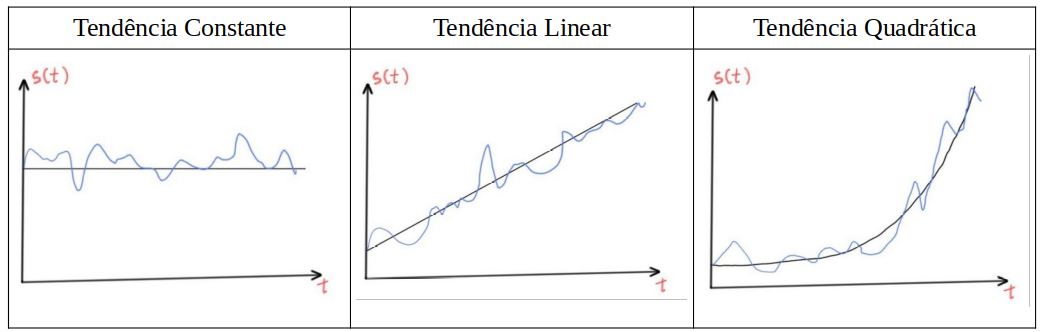
\includegraphics[width=.9\linewidth]{tendencias.png} 
    \label{fig:tendenciaSerie}
\end{figure}

A tendência de uma série temporal é utilizada para descrever o comportamento da série ao longo do tempo, ou seja, verifica se há uma inclinação de alta, queda ou nula, além de indicar a velocidade dessas mudanças. Desse modo, existem diferentes formas matemáticas representativas destes movimentos da série temporal, como pode ser verificado na Figura \ref{fig:tendenciaSerie}. A tendência constante é aquela em que a série apresenta um comportamento linear ao longo do tempo, sem variações significativas. A tendência linear, por sua vez, é aquela em que a série apresenta uma inclinação de alta ou queda ao longo do tempo. Já a tendência quadrática é aquela em que a série apresenta uma curvatura ao longo do tempo, podendo assumir comportamentos de concavidade para cima ou para baixo. 

Já os ciclos são componentes de uma série temporal que visam identificar padrões que se repetem regularmente em um curto intervalo de tempo. Eles são caracterizados por movimentos cíclicos em torno da tendência com duração de períodos variáveis como pode ser visualizado na Figura \ref{fig:ciclos}. Os ciclos são afetados por fatores externos, como mudanças econômicas, políticas, climáticas ou outros aspectos que regem a série abordada, e geralmente não são previsíveis a longo prazo.


\begin{figure}[htbp]
     \centering
     \caption{Características cíclicas e sazonais de uma série temporal.}
     \begin{subfigure}[b]{0.46\textwidth}
         \centering
         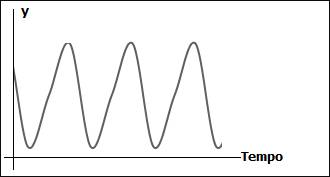
\includegraphics[width=.99\linewidth, height=3.5cm]{ciclos.jpg}
         \caption{Ciclos em uma série temporal.}
         \label{fig:ciclos} 
     \end{subfigure}
     \hfill
     \begin{subfigure}[b]{0.495\textwidth}
         \centering
         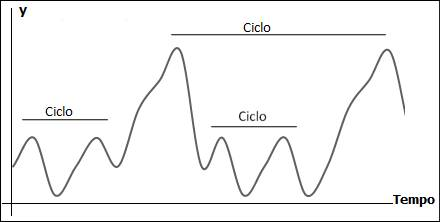
\includegraphics[width=.99\linewidth, height=3.5cm]{sazonais.jpg}
         \caption{Períodos sazonais.}
         \label{fig:sazonalidade}
     \end{subfigure}

     Fonte: \citeonline{Waldir}.
\end{figure}

Por fim, entende-se a sazonalidade como as variações regulares que ocorrem em uma série temporal em intervalos fixos de tempo, como dias, semanas, meses ou anos. Um exemplo disso pode ser observado na Figura \ref{fig:sazonalidade}, em que um padrão visual é repetido em um determinado intervalo de tempo. Essas variações podem ser influenciadas por fatores sazonais, como clima, feriados, eventos culturais, entre outros. A sazonalidade é uma componente importante de muitas séries temporais, e sua identificação é fundamental para uma análise precisa dos dados. A principal diferença entre componentes cíclicas e sazonais é que, enquanto nas cíclicas os movimentos são mais difíceis de prever, pois tendem a ser irregulares, na sazonalidade os movimentos ocorrem em intervalos regulares no tempo, tornando-os mais previsíveis. 

\section{Mercado Financeiro}
\label{subsec:mercado_financeiro}
O mercado financeiro é um ambiente de negociação de diversos ativos financeiros, tais como ações, títulos, moedas, commodities e derivativos. Ele é composto por instituições financeiras, investidores, empresas, governos e outros agentes econômicos, que buscam negociar esses ativos visando lucros, proteção contra riscos e diversificação de investimentos. Os investidores (credores), que fornecem capital para o mercado financeiro, podem ser tanto pessoas físicas como jurídicas e podem investir em diferentes tipos de ativos, dependendo de seus objetivos, perfil de risco e estratégia. Já os capitadores (mutuários), que captam recursos, podem ser empresas, governo ou outras instituições que buscam financiamento para seus projetos ou operações \cite{mercado}. As negociações no mercado financeiro geram uma grande quantidade de dados, que podem ser organizados e analisados como séries temporais devido a característica gradual e temporal do sistema, permitindo a identificação de tendências, ciclos e sazonalidades nos preços dos ativos ao longo do tempo. 

Para facilitar a análise de séries temporais no mercado financeiro, conceitos como o gráfico de velas apresentado na Figura \ref{fig:grafico_velas} tem sido amplamente adotado, pois consegue discretizar os dados de acordo com uma granulação sem perda de informações relevantes para as partes envolvidas \cite{bulkowski2012encyclopedia}. Através deste gráfico, é possível obter informações como valor de abertura, valor máximo, valor mínimo e valor de fechamento de cada instante $t$ de tempo, caracterizado do inglês \ac{OHLC}. Tais elementos podem ser observadas na Figura \ref{fig:candle_definition}. Além disso, outra informação relevante que pode ser correlacionada com esse gráfico é o volume de transações, que indica momentos de forte movimento no mercado ou baixa capacidade de conversão de capital. Respaldado nessas informações, os investidores podem tomar decisões mais informadas sobre quando comprar ou vender ativos financeiros, buscando maximizar seus lucros e minimizar os riscos de seus investimentos.

\begin{figure}[htbp]
     \centering
     \caption{Gráfico de velas e suas características observáveis.}
     \begin{subfigure}[b]{0.48\textwidth}
         \centering
         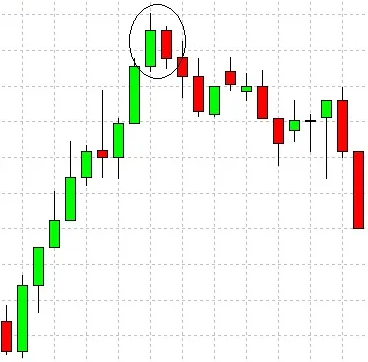
\includegraphics[width=\linewidth, height=3.8cm]{grafico_velas.png}
         \caption{Representação de série temporal em gráfico de velas.}
         \label{fig:grafico_velas} 
     \end{subfigure}
     \hfill
     \begin{subfigure}[b]{0.48\textwidth}
         \centering
         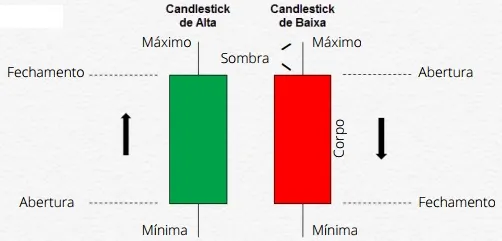
\includegraphics[width=\linewidth, height=3.8cm]{candlestick.png}
         \caption{Padrões observáveis em um candle.}
         \label{fig:candle_definition}
     \end{subfigure}

     Fonte: \citeonline{trade_mental:2022}.
\end{figure}
Com base no modelo de gráfico de velas e na forma que os dados são discretizados em \ac{OHLC}, surgiram diversas abordagens com o objetivo de obter melhores resultados no contexto de investimentos. Entre esses métodos, as alternativas baseadas em \ac{IA} têm despertado grande interesse, devido à sua capacidade de identificar padrões complexos \cite{dwivedi2021artificial}. Essa abordagem utiliza algoritmos de \ac{IA} e dados históricos para analisar os padrões de mercado e tomar decisões de investimento de forma mais precisa e automatizada. Esses algoritmos são capazes de aprender com os dados históricos e adaptar suas estratégias com base nas mudanças da série temporal selecionada, oferecendo assim um potencial de obtenção de retornos superiores a média \cite{strader2020machine}.

\section{Abordagens}
\label{subsec:abordagem}
Na tarefa de previsão da tendência ou do preço de um determinado ativo, uma variedade de técnicas podem ser empregadas. Entre elas, destacam-se a análise gráfica \cite{matsura2017comprar}, análise de sentimento \cite{igarashi2021analise} e análise fundamentada em dados numéricos \cite{halil2019predicting}, esta última sendo o foco dos trabalhos analisados. Para isso, tais estudos seguem em sua maioria uma abordagem padrão, conforme ilustrado na Figura \ref{fig:abordagemPadrao}. Nesse processo, a primeira etapa consiste na extração de dados que apresentam uma boa correlação com a saída desejada, sendo essa etapa detalhada na Seção \ref{subsec:conjunto_dados}. Em seguida, são geradas novas variáveis por meio de modelos matemáticos, visando obter representações aprimoradas do problema no domínio temporal. As formulações matemáticas utilizadas para essa geração de variáveis podem ser encontradas na Seção \ref{subsec:geracao_novas_variaveis}. Posteriormente, ocorre a seleção de variáveis, empregando métodos estatísticos determinísticos e não determinísticos, incluindo modelos de \ac{IA}, que são explorados com mais detalhes na Seção \ref{subsec:selecao_variaveis}. Considerando que os estudos mencionados podem incorporar algumas ou todas as etapas da abordagem padrão (Figura \ref{fig:abordagemPadrao}), também foi observado em alguns trabalhos a utilização da normalização dos dados, com o objetivo de padronizar todos os valores em uma mesma escala.

\begin{figure}[htbp]
    \caption{Processo de desenvolvimento dos trabalhos analisados.}
      \centering
      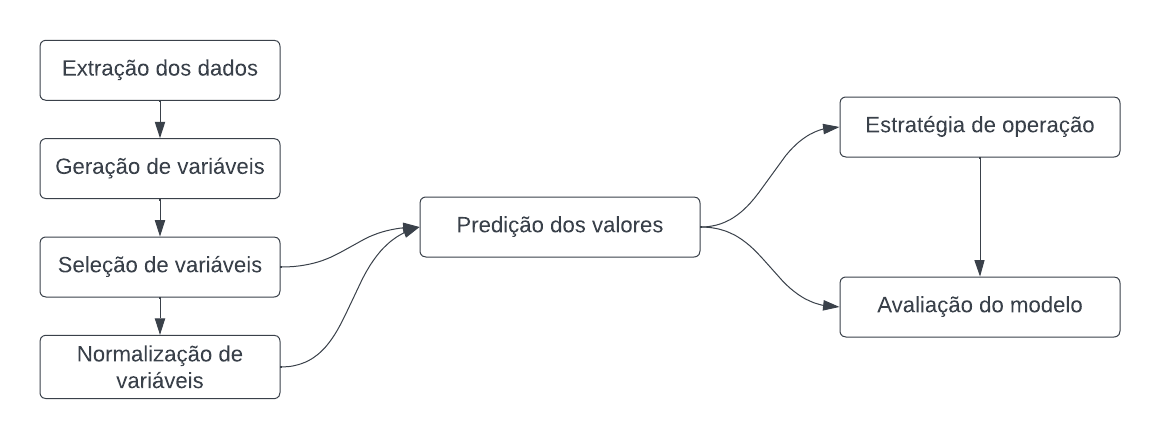
\includegraphics[width=.9\linewidth]{fluxo_abordagem.png} 
    \label{fig:abordagemPadrao}
\end{figure}

Com as variáveis selecionadas, inicia-se o processo de treinamento dos modelos utilizados em cada trabalho, conforme descrito na Seção \ref{subsec:tecnicas_predicao}. Após a obtenção dos resultados das previsões por meio desses modelos, é possível realizar uma análise mais aprofundada do seu desempenho. Alguns trabalhos utilizam a técnica de comitê (\textit{ensemble}) que tende a aumentar a capacidade do modelo resultante \cite{sagi2018ensemble}. Além disso, a ação final tomada com base nas previsões pode variar de acordo com os objetivos do pesquisador. Os métodos utilizados nessa etapa são abordados na Seção \ref{subsec:estrategias}. Por fim, realiza-se uma análise do resultado por meio de métricas estatísticas, a fim de medir o desempenho do modelo ou da estratégia utilizada. Tais métricas são apresentadas na Seção \ref{subsec:criterio_avaliacao}. 



\section{Conjuntos de Dados}
\label{subsec:conjunto_dados}
A qualidade e a quantidade de dados utilizados no treinamento do modelo de previsão, desempenham um papel fundamental na obtenção de resultados positivos. Para alcançar bons desdobramentos na tarefa de previsão, é necessário garantir que o conjunto de dados seja representativo da realidade e abranja o maior número possível de características do ativo financeiro em questão \cite{kumar2020data}. Além disso, é importante realizar um pré-processamento adequado dos dados antes de utilizá-los no treinamento do modelo, pois a presença de dados incompletos, incorretos ou inconsistentes pode afetar a assertividade das previsões \cite{kaur2019systematic}.

Nesse sentido, técnicas de pré-processamento de dados são frequentemente aplicadas para lidar com esses problemas. Essas técnicas incluem a imputação de dados faltantes, a remoção de \textit{outliers}, a padronização e normalização dos dados, a redução de dimensionalidade e a geração de novas variáveis por meio de cálculos matemáticos \cite{tomasevic2020overview}. A escolha adequada do conjunto de dados e a aplicação correta das técnicas de pré-processamento são fatores determinantes para o sucesso da previsão utilizando métodos inteligentes.

Os estudos analisados nesta pesquisa utilizam dados brutos do volume de transação e \ac{OHLC} em diversas granularidades, como minutos, horas ou dias. Por se tratar de uma série temporal, é comum que esses dados sejam coletados de forma contínua, sem lacunas ou dados faltantes. É importante ressaltar que a remoção de amostras não é recomendada, uma vez que a ordem das amostras é um fator crucial na construção das séries temporais. Além disso, outras variáveis são geradas a partir de cálculos matemáticos realizados com base nessa série, como descrito na Seção \ref{subsec:geracao_novas_variaveis}.

Certos trabalhos analisados nesta pesquisa optam por normalizar os dados, a fim de colocar os valores das variáveis dentro de um limite específico e reduzir as diferenças desproporcionais entre elas. Alguns pesquisadores realizam a normalização devido à capacidade do algoritmo em lidar apenas com dados normalizados \cite{Manrui_two-stage}, enquanto outros aplicam essa técnica por terem observado melhorias nos resultados após a normalização \cite{Anand_Comparison, Chaojie_Stock}. É importante ressaltar que existem várias maneiras de normalizar um conjunto de dados, sendo as técnicas mais comuns a \textit{Min-Max} \cite{Leonardo_Comparative, Gourav_Swarm}, o \textit{Z-Score} \cite{fei2021z}, a normalização por escala decimal \cite{patro2015normalization}, entre outras, que delimitam os valores dentro de um intervalo, geralmente de -1 a 1 ou 0 a 1 \cite{Jerzy_Deep}. Portanto, a normalização dos dados pode ser uma etapa essencial para permitir que o modelo compreenda melhor as relações entre as variáveis e, assim, realize previsões mais precisas.



\section{Geração de Variáveis}
\label{subsec:geracao_novas_variaveis}
Para melhorar o desempenho dos modelos, algumas abordagens utilizam técnicas de geração de variáveis adicionais derivadas dos dados brutos. Os métodos de geração de novos dados a partir dos dados brutos de \ac{OHLC} são amplamente utilizados para fornecer informações adicionais sobre o ativo financeiro em questão.

Do conjunto de modelos matemáticos existentes com a capacidade de gerar dados relevantes para a previsão de valores de ativos financeiros, destacam-se dentre os trabalhos analisados:

\begin{itemize}
    \item \ac{VP} - estabelece intervalos temporais conhecidos como janelas, abrangendo dados anteriores ao ponto de análise \cite{vinicius_sistemas, gabriel2023neo}, tais como $S_{t-1}, S_{t-2}, ..., S_{t-n}$, em que $S_{t-1}$ representa o valor da série temporal no instante $t-1$ e $n$ é o tamanho da janela.
    
    \item \ac{SMA} - um modelo matemático utilizado para suavizar a flutuação dos dados de preço ao longo do tempo e identificar tendências de forma mais clara \cite{vinicius_sistemas, Ciniro_Econometric}. A \ac{SMA} pode ser obtida por:
    \begin{equation}
    \label{eq:SMA}
        SMA = \frac{1}{n} \sum_{i=0}^{n-1} S_{t-i},
    \end{equation}
    em que $n$ é o tamanho da janela móvel e $S_{t-i}$ representa o valor da série temporal no instante $t-i$.
    
    \item \ac{EMA} - um modelo matemático semelhante ao \ac{SMA}, porém com mais peso atribuído aos preços mais recentes, tornando-o mais sensível às mudanças recentes nos dados \cite{Charlene}. O \ac{EMA} é calculado conforme:
    \begin{equation}
        \label{eq:EMA}
        EMA = \alpha (S_t - EMA_{t-1}) + EMA_{t-1},
    \end{equation}
    em que $S_t$ é o valor da série temporal no instante $t$, $\alpha$ é o fator de suavização (frequentemente definido como $\alpha = \frac{2}{n+1}$) e $EMA_{t-1}$ representa o valor do \ac{EMA} no instante $t-1$.
    
    \item \ac{MACD} - identifica a direção e força de uma tendência predominante em um ativo financeiro \cite{C_Veeramani_Exploration}. O cálculo deste indicador é dado por: 
    \begin{equation}
        \label{eq:MACD}
        MACD = EMA(w) - EMA(k),
    \end{equation}
    em que $w$ é a janela móvel curta e $k$ é a janela móvel longa.
    
    \item \ac{CCI} - identifica pontos de reversão de tendência e avalia sua força \cite{altan2019effect, halil2019predicting}. O cálculo deste indicador é realizado da seguinte forma:
    \begin{equation}
        \label{eq:CCI}
        CCI = \frac{TP - SMA(TP,c)}{0.015 \times DP(TP)},
    \end{equation}
    em que $n$ é a janela de amostragem desejada, $DP$ representa o desvio padrão da série e $TP$ é calculado como $TP = \frac{C+H+L}{3}$, em que $H$ é o ponto de máximo, $L$ é o ponto de mínimo e $C$ é o valor de fechamento do \textit{candle} atual. 
    
    \item \ac{ADX} - avalia a força de uma tendência predominante em um ativo financeiro, independentemente de sua direção \cite{gao2021stock}. Este índice é calculado como se segue: 
    \begin{equation}
        \label{eq:ADX}
        ADX = \frac{(n-1) \times EMA(TR) + TR}{n},
    \end{equation}
    em que $n$ indica a janela de amostragem desejada e $TR$ é obtido através de $TR = \max(H-L, |H-C_{t-1}|, |L-C_{t-1}|)$, em que $H$ é o ponto de máximo do \textit{candle} atual, $L$ é o ponto de mínimo e $C_{t-1}$ representa o valor de fechamento do \textit{candle} anterior.
    
    \item \ac{ROC} - mede a variação percentual de preço do ativo ao longo de um determinado período de tempo \cite{ampomah2020evaluation, jiang2020improved}. Este indicador é computado por: 
    \begin{equation}
        \label{eq:ROC}
        ROC = \frac{S_{t}-S_{t-n}}{S_{t-n}} \times 100,
    \end{equation}
    considerando apenas o valor atual $S_t$ e o valor de $n$ estados passados $S_{t-n}$ da série temporal.
    
    \item \ac{TSI} - identifica a força e a direção de uma tendência em um determinado ativo financeiro, combinando a suavização do \ac{EMA} com a taxa de variação \ac{ROC} dos preços para fornecer sinais de compra e venda \cite{anwar2019forecasting}. Este índice é obtido através da seguinte fórmula:     
    \begin{equation}
        \label{eq:TSI}
        TSI = \frac{EMA(EMA(PC,w), k)}{EMA(EMA(|PC|,w), k)} \times 100,
    \end{equation}
    em que $PC$ representa a variação do preço de fechamento ($C_{t-1} - C_t$), $w$ é a janela móvel curta e $k$ é a janela móvel longa.
    
    \item \ac{K} - identifica a condição de sobre-compra e sobre-venda de um ativo financeiro, fornecendo sinais de compra e venda com base em movimentos de preço em relação à sua faixa de preço recente \cite{Leonardo_Comparative, C_Veeramani_Exploration}. Podendo ser calculado pela equação a seguir: 
    \begin{equation}
        \label{eq:K}
        \%K = \frac{C_t-L_{t-n}}{H_{t-n}-L_{t-n}},
    \end{equation}
    em que $C_t$ é o valor de fechamento atual, $L_{t-n}$ e $H_{t-n}$ são o valor mínimo e máximo de $n$ \textit{candles} passados.
    
    \item \ac{D} - é uma média móvel de $n$ períodos do \%K, utilizada para fornecer um sinal mais suave e reduzir a volatilidade dos resultados \cite{Leonardo_Comparative, C_Veeramani_Exploration}. O \ac{D} é obtido por:
    \begin{equation}
        \label{eq:D}
        \%D = \frac{\sum_{i=0}^{n-1}\%K_{t-i}}{n},
    \end{equation}
    em que $\%K_{t-i}$ é o valor de \%K no instante $t-i$.

    \item \ac{R} - assim como o indicador \ac{K}, esse método tem como objetivo identificar condições de sobre-compra e sobre-venda de um ativo financeiro, porém com escalas invertidas \cite{lee2021exploring}. É calculado pela seguinte equação: 
    \begin{equation}
        \label{eq:R} 
        \%R = \frac{H_{t-n}-C_t}{H_{t-n}-L_{t-n}},
    \end{equation}
    onde $C_t$ é o valor de fechamento atual, $L_{t-n}$ e $H_{t-n}$ representam o valor mínimo e máximo de $n$ \textit{candles} passados. 
\end{itemize}


É importante observar que muitos dos métodos mencionados anteriormente podem ser empregados como modelos de predição. No entanto, este trabalho não se concentra nessa abordagem, uma vez que não é o foco da pesquisa.

\section{Seleção de Variáveis}
\label{subsec:selecao_variaveis}
A seleção de variáveis desempenha um papel crucial no modelo de IA, pois um grande número de variáveis pode dificultar o treinamento e levar ao \textit{overfitting}, prejudicando o desempenho do modelo. Apesar do processo de extração e criação gerar muitas variáveis descritivas, nem todas são igualmente úteis para a previsão, e a seleção de variáveis permite concentrar-se nos aspectos mais importantes e relevantes para essa tarefa \cite{meyer2019importance}.
Para isso, existem diversos métodos de seleção de variáveis, alguns voltados especificamente para a atividade de classificação, enquanto outros podem ser aplicados tanto para classificação quanto para regressão. Esses métodos auxiliam na identificação das variáveis mais relevantes e descartam aquelas que têm pouca influência no modelo final. 

Uma parte dos trabalhos analisados utilizou métodos de seleção específicos para o problema de classificação. Dentre esses métodos, destacam-se:
\begin{itemize}
    \item \textit{Fisher} - aplicado por \citeonline{peng2021feature}, que calcula o escore de \textit{Fisher} para selecionar as características mais importantes com base na separação entre as classes \cite{fisher1936use};

    \item  \textit{Gini} - empregado por \citeonline{ji2022adaptive}, que calcula o índice de impureza de \textit{Gini} para cada \textit{feature} em relação à variável de saída, sendo selecionadas aquelas com maior poder discriminativo \cite{gini1921measurement}; 

    \item \ac{R2} - utilizado por \citeonline{gabriel2023neo}, que determina se existe uma relação significante entre duas variáveis categóricas, auxiliando na seleção das características mais informativas para a classificação \cite{pearson1900x}.
\end{itemize}
 Esses métodos contribuem para identificar as características mais relevantes e reduzir a dimensionalidade do conjunto de dados, melhorando a eficiência e a interpretabilidade dos modelos de classificação.

Para abranger a classe dos algoritmos de regressão, foram utilizados diversos métodos de seleção de variáveis. Entre eles, foram empregadas abordagens estocásticas, que visam encontrar o melhor conjunto de variáveis por meio de métodos não-determinísticos, representados pelos modelos de IA. Esses métodos treinam uma determinada rede e avaliam qual conjunto de variáveis foi mais eficiente para a tarefa de previsão. Nesse contexto, os métodos mais utilizados foram: 
\begin{itemize}
    \item \ac{RF} aplicado por \citeonline{Amin_Aminimehr_Comprehensive}, que gera várias combinações de entradas de forma aleatória e treina uma árvore de decisão para cada combinação, selecionando assim as variáveis da árvore que obtêm os melhores resultados \cite{breiman2001random}; 
    \item Lasso empregado por \citeonline{sermpinis2018modelling}, que separa as melhores variáveis com base em seus pesos na tarefa de previsão, zerando o peso das variáveis menos relevantes \cite{muthukrishnan2016lasso}; 
    \item ElasticNet adotado por \citeonline{zhang2023forecasting}, que combina as técnicas de regularização L1 (Lasso) e L2 (Ridge), gerando assim um vetor ponderado pelo nível de significância de cada variável \cite{amini2021two}.
\end{itemize}
É importante ressaltar que há também métodos determinísticos baseados em conceitos estatísticos para essa tarefa, como o teste de \textit{Kruskal-Wallis}, utilizado por \citeonline{vinicius_sistemas}, que compara as medianas de duas ou mais amostras independentes para determinar se há diferença estatisticamente significativa entre elas \cite{kruskal1952use}; e o método de \ac{RIM}, empregado por \citeonline{zhao2019maximum}, que mede a dependência mútua entre cada recurso e a variável de destino, utilizando a entropia da informação \cite{kraskov2004estimating}.

\section{Técnicas de Predição}
\label{subsec:tecnicas_predicao}
Existem diversas abordagens para o processo de predição de valores, desde modelos lineares até modelos não lineares. Cada uma dessas abordagens possui suas próprias características e cenários de atuação, resultando em um bom desempenho de alguns em relação a outros em cenários específicos. No entanto, não é possível afirmar que uma abordagem é totalmente superior à outra, uma vez que a escolha depende do problema em questão e dos dados disponíveis. Dentre os métodos exploradas, pode-se citar as abordagens estatísticas, modelos baseados em \ac{IA}.

Dentro da classe de modelos estatísticas, são exploradas diferentes abordagens para realizar previsões e análises. Além de ajustes lineares que buscam a linearidade local na vizinhança \cite{Charlene} e o uso de \ac{SMA} \cite{Ciniro_Econometric}, também são empregados métodos como \ac{ARIMA} \cite{Leonardo_Comparative, gao2021stock}, \ac{SARIMA} e \ac{GARCH} \cite{Ciniro_Econometric}. O modelo \ac{ARIMA} combina elementos de autoregressão (AR), média móvel (MA) e diferenciação (I) para modelar padrões temporais e sazonalidade, enquanto o \ac{SARIMA} incorpora componentes de sazonalidade em adição aos componentes de tendência e aleatoriedade. Já o modelo \ac{GARCH} é usado para modelar a volatilidade condicional em séries temporais financeiras, capturando a natureza heterocedástica dos retornos. É importante ressaltar que muitos desses modelos estatísticos são utilizados em conjunto com abordagens de \ac{IA}, permitindo explorar as vantagens de cada modelo e obter previsões mais precisas e confiáveis \cite{Ciniro_Econometric}.

Já a classe de \textit{machine learning}\footnote{Modelos de Machine Learning são algoritmos e sistemas que aprendem padrões a partir de dados, permitindo que uma máquina tome decisões ou faça previsões sem ser explicitamente programada para uma tarefa específica. Esses modelos podem ser supervisionados, não supervisionados ou por reforço, dependendo do tipo de aprendizado envolvido.} foi amplamente explorada nos trabalhos analisados, abrangendo uma variedade de modelos com diferentes naturezas. Dentre os modelos de natureza linear, destacam-se o uso do \ac{SVM} \cite{altan2019effect, Anand_Comparison} e \ac{LR} \cite{pabucccu2023forecasting}. Além disso, foram investigados modelos de natureza não linear, como \ac{MLP} \cite{Jerzy_Deep, Faramarz_Integrating}, \ac{ELM} \cite{Manrui_two-stage}, \ac{EGNN}, \ac{EMG}, \ac{EOGS} \cite{vinicius_sistemas}, \textit{WaveNet} \cite{Leonardo_Comparative}, \ac{SVR}, \ac{RBF}, \ac{ANFIS} \cite{Faramarz_Integrating}, \ac{DT} e \ac{KNN}\cite{halil2019predicting}. Essa diversidade de modelos mostra a abrangência das abordagens de \textit{machine learning} utilizadas nos estudos, permitindo explorar tanto a linearidade quanto a não linearidade dos dados para obter previsões mais precisas e acuradas.

Por fim, os modelos de \textit{deep learning}\footnote{Deep Learning é uma subárea do Machine Learning que utiliza redes neurais artificiais profundas para realizar tarefas complexas de aprendizado e reconhecimento de padrões. Essas redes, inspiradas no funcionamento do cérebro humano, consistem em várias camadas de neurônios interconectados, permitindo a extração automática de características hierárquicas dos dados.} despertaram grande expectativa nos estudos analisados, devido à sua capacidade de reconhecer padrões complexos. Foram empregados diversos modelos, como \ac{LSTM} \cite{anwar2019forecasting, Xiaoci_Predicting, Jian_Forecasting, gao2021stock,  lee2021exploring, Firat}, \textit{Transformer} \cite{Chaojie_Stock}, \ac{CNN} \cite{Anand_Comparison}, \ac{RNN} \cite{Xiaoci_Predicting, gao2021stock, Anand_Comparison, Firat}, \ac{TCN} \cite{Firat}, \ac{DBN} \cite{Xiaoci_Predicting}, \ac{DCFS} \cite{Li-Xin_Fast} e \ac{DCDNN} \cite{Jian_Forecasting}. Essa variedade de modelos demonstra a ampla gama de técnicas de \textit{deep learning} aplicadas, explorando a capacidade dessas redes neurais em capturar informações de longo prazo, realizar análises sequenciais e lidar com dados de alta complexidade. 

\section{Estratégias}
\label{subsec:estrategias}

Após a previsão do valor de um ativo específico, torna-se possível tomar uma decisão embasada, e para isso, os estudos analisados apresentam diversas estratégias distintas com o objetivo de maximizar o retorno durante as operações. 

Uma pesquisa conduzida por \citeonline{SALMAN2012regression} demonstrou a possibilidade de transformar modelos de regressão em modelos de classificação com base em três regras similares apresentadas na Tabela \ref{tab:RegraTransf}. Nesta abordagem, a classe -1 indica uma tendência de queda, 0 indica ausência de tendência, e 1 representa uma tendência de alta para a interação em questão. 

\begin{table}[h]
\begin{center}
\begin{tabular}{ccc}
\hline
Exemplo            & Regra                   & Classe \\ \hline
\multirow{2}{*}{A} & $Y_{t} > Y_{t-1}$    & 1      \\
             & $Y_{t} =Y_{t-1}$              & 0      \\
             & $Y_{t} < Y_{t-1}$       & -1     \\ \hline
\multirow{2}{*}{B} & $Y_t \geq Y_{t-1}$ & 1      \\
             & $Y_t < Y_{t-1}$       & -1     \\ \hline
\multirow{2}{*}{C} & $Y_t > Y_{t-1}$    & 1      \\
             & $Y_t \leq Y_{t-1}$    & -1     \\ \hline
\end{tabular}
\end{center}
\caption{Transformação da saídas no domínio contínuo para o domínio discreto.}
\label{tab:RegraTransf}
\end{table}

Nesse sentido, alguns estudos exploraram modelos robustos de regressão para, posteriormente, converter as saídas em classes de alta, baixa ou até mesmo constância dos valores \cite{ampomah2020evaluation, jiang2020improved, Xiaoci_Predicting}. Essa abordagem permite uma interpretação mais direta e prática dos resultados, facilitando a tomada de decisões e a implementação de estratégias de investimento. Ao transformar as previsões em classes, os modelos podem fornecer informações sobre a direção do movimento do ativo financeiro, indicando se é provável que ele aumente, diminua ou permaneça estável. 

Estratégias baseadas em classificação geralmente adotam a abordagem de compra quando o retorno é classificado como positivo e venda quando o retorno é classificado como negativo \cite{Chaojie_Stock}. Em alguns estudos que utilizam essa técnica, essas operações são executadas com todo o capital disponível na carteira de investimentos \cite{Jerzy_Deep, Charlene, C_Veeramani_Exploration}.

No trabalho desenvolvido por \citeonline{Ciniro_Econometric}, não é utilizado apenas um modelo de previsão, mas sim uma combinação de diferentes preditores. Para lidar com essa situação, estratégias são desenvolvidas para integrar as saídas desses diversos modelos de forma a maximizar os resultados obtidos. Portanto, foi criado um modelo de comitê (\textit{ensemble}) para tomar decisões com base nas previsões dos modelos individuais. Nesse trabalho, são apresentadas três regras para obter o sinal final. A primeira regra é a \ac{ADC}, que verifica se os resultados dos modelos do comitê coincidem em relação à tendência (subir ou descer). Se os modelos indicarem a mesma direção, um sinal de subir ou descer é gerado; caso contrário, um sinal estável é retornado. A segunda regra é a \ac{MDC}, que considera a contagem de votos e gera um sinal de subir ou descer se houver uma maioria de votos concordantes. Caso contrário, um sinal estável é retornado. Por fim, temos a \ac{AMC}, que verifica se as duas regras anteriores estão em acordo. Se os resultados forem semelhantes, um sinal de subir ou descer é gerado; caso contrário, um sinal estável é gerado. Com base na saída da regra \ac{AMC}, é possível decidir entre comprar ou vender o ativo financeiro. Essa escolha é feita de acordo com a interpretação do sinal gerado pela regra. Quando a saída indica um sinal de compra, significa que há uma tendência de alta no ativo, o que pode ser um momento favorável para realizar uma compra. Por outro lado, quando a saída indica um sinal de venda, significa que há uma tendência de queda no ativo, o que pode ser apropriado para realizar uma venda.


\section{Critérios de Avaliação}
\label{subsec:criterio_avaliacao}
As ferramentas de análise são responsáveis por fornecer parâmetros de comparação e visualização do desempenho das abordagens. Para tal, dois ramos da análise estatística são direcionados à tarefa de previsão com modelos de \ac{IA}: a análise de problemas de classificação e a análise de problemas de regressão. A análise de problemas de classificação é voltada para a previsão de eventos discretos, como a indicação de compra ou venda de uma ação. Já a análise de problemas de regressão é voltada para previsão de valores contínuos, como o preço de uma ação em um determinado momento.

\begin{figure}[htbp]
    \caption{Matriz de confusão.}
      \centering
      \includegraphics[width=.6\linewidth]{matriz_confusão.png} 
    \label{fig:matrizconfusao}
\end{figure}

Para avaliar a efetividade dos modelos de classificação, é comum utilizar métricas que mensurem a quantidade de classificações corretas, tais como:
\begin{itemize}   
    \item Precisão Positiva e Negativa - são métricas que medem a capacidade de um modelo em identificar corretamente amostras positivas e negativas, respectivamente \cite{Xiaoci_Predicting}. Essas métricas são calculadas usando uma matriz de confusão, que compara as classificações do modelo com as classes verdadeiras dos dados. A matriz de confusão pode ser visualizada na Figura \ref{fig:matrizconfusao}. A equação para o calculo da \ac{PP}, utiliza os dados de \ac{TP} e \ac{FP}, sendo descrita como: 
    \begin{equation}
        \label{eq:PP}
        PP = \frac{TP}{TP+FP}.
    \end{equation}
    Já para calcular a \ac{PN}, utiliza-se os valores de \ac{TN} e \ac{FN} conforme:
    \begin{equation}
        \label{eq:PN}
        PN = \frac{TN}{TN + FN}.
    \end{equation}

    \item \textit{Recall} - é uma métrica que mede a proporção de amostras positivas corretamente identificadas pelo modelo em relação ao total de amostras positivas presentes nos dados reais. Em outras palavras, o \textit{recall} indica a capacidade do modelo de "lembrar"  corretamente das amostras positivas \cite{ampomah2020evaluation}. Tal método pode ser calculado por: 
    \begin{equation}
        \label{eq:recall}
        Recall = \frac{TP}{TP + FN}.
    \end{equation}
    
    \item \ac{AC} - mede a proporção de amostras classificadas corretamente em relação ao total de amostras \cite{ampomah2020evaluation, vinicius_sistemas, lee2021exploring}. A fórmula para o cálculo da \ac{AC} é dada por:
    \begin{equation}
        \label{AC}
        AC = \frac{TP + TN}{TP + TN + FP + FN}.
    \end{equation}    
\end{itemize}

Note que a acurácia (AC) pode ser enganosa em conjuntos de dados desbalanceados, nos quais uma classe é predominante. Nesses casos, um modelo pode obter uma alta taxa de acertos simplesmente prevendo a classe predominante para todas as amostras. Para lidar com esse problema, é necessário utilizar outra métrica que avalia o desempenho dos modelos de classificação em termos de sensibilidade e equilíbrio entre Precisão e \textit{Recall}, tal como o \ac{F1} que é uma média harmônica da \ac{PP} e do \textit{Recall}. Essa métrica fornece uma medida única de desempenho de um modelo de classificação, equilibrando a importância tanto da \ac{PP} quanto do \textit{Recall} \cite{jiang2020improved}. O calculo da \ac{F1} é dada por: 
\begin{equation}
  \label{eq:F1}
  F1 = 2 \frac{PP  \textit{Recall}}{PP + \textit{Recall}}.
\end{equation}

Já para os modelos de regressão, a efetividade é mensurada de diferentes formas, uma vez que é muito improvável obter a previsão exata do valor de saída. Nesse contexto, os trabalhos analisados utilizam das seguintes métricas: 

\begin{itemize}
    \item \ac{R²} - é uma medida da qualidade do ajuste do modelo aos dados observados \cite{Charlene, Jian_Forecasting}. O valor de R² varia de 0 a 1, indicando a proporção de variabilidade explicada pelo modelo e é dado por:
    \begin{equation}
        \label{R²}
        R^2 = 1- \left(\frac{SSE}{SST}\right),
    \end{equation}
    sendo que $SSE$ é a soma dos quadrados dos resíduos do modelo, que representa a variação não explicada pelo modelo de regressão e o $SST$ é a soma dos quadrados totais, que representa a variação total da variável dependente.
    
    \item \ac{ME} - verifica se as previsões estão consistentemente superestimando ou subestimando os valores reais \cite{Leonardo_Comparative}. Pode ser calculado por:
    \begin{equation}
        \label{eq:ME}
        ME = \frac{1}{n} \sum(y_{pred} - y_{real}),
    \end{equation}
    no qual $n$ é a quantidade de amostras, $y_{pred}$ é o valor predito pelo modelo e $y_{real}$ é a saída desejada.
    
    \item \ac{MAE} - quantifica o erro médio entre as previsões e os valores reais de uma variável sem se importar com o sentido do erro \cite{Amin_Aminimehr_Comprehensive, Manrui_two-stage}. O \ac{MAE} pode ser obtido por:
    \begin{equation}
        \label{eq:MAE}
        MAE = \frac{1}{n} \sum(|y_{pred} - y_{real}|).
    \end{equation}
    
    \item \ac{MSE} - avalia a dispersão das previsões em relação aos valores reais, penalizando erros maiores de forma quadrática \cite{Jian_Forecasting, Chaojie_Stock}. O \ac{MSE} é calculado por:
    \begin{equation}
        \label{eq:MSE}
        MSE = \frac{1}{n} \sum(y_{pred} - y_{real})^2.
    \end{equation}
    
    \item \ac{MAPE} - avalia a precisão de um modelo de previsão em termos percentuais \cite{Anand_Comparison, Firat}. O \ac{MAPE} pode ser obtido por:
    \begin{equation}
        \label{eq:MAPE}
        MAPE = \frac{1}{n} \sum \left | \frac{y_{pred} - y_{real}}{y_{real}} \right | 100.
    \end{equation}
    
    \item \ac{RMSE} - mede a diferença entre os valores previstos por um modelo e os valores reais, sendo expressa na mesma unidade dos valores originais \cite{altan2019effect, pabucccu2023forecasting}. O \ac{RMSE} é calculado por:
    \begin{equation}
        \label{eq:RMSE}
        RMSE = \sqrt{\frac{1}{n} \sum(y_{pred} - y_{real})^2}.
    \end{equation}
\end{itemize}


É importante ressaltar que diversos estudos analisaram os modelos por meio dos resultados obtidos após a aplicação da estratégia de investimento, utilizando uma variedade de métricas econômicas. Essas métricas incluem o retorno financeiro, a comparação do desempenho do modelo em relação à estratégia \textit{buy and hold} (comprar e manter) \cite{Ciniro_Econometric}, o retorno percentual do valor investido \cite{Chaojie_Stock}, a avaliação do lucro e perda, o retorno anual esperado \cite{Charlene}, o número de transações realizadas, o número de operações rentáveis \cite{C_Veeramani_Exploration}, o número de transações rentáveis consecutivas, a perda bruta e o lucro bruto \cite{Jerzy_Deep}. Essas métricas fornecem uma avaliação abrangente do desempenho dos modelos em termos de rentabilidade, consistência e eficácia na tomada de decisões de investimento. Além disso, no contexto da avaliação de desempenho dos modelos, também é possível aplicar testes estatísticos, como o T-test \cite{kim2015t}, teste de McNemar \cite{mcnemar1947note}, teste de Friedman \cite{sheldon1996use}, entre outros, a fim de obter uma análise estatisticamente significativa dos resultados.

\section{Resumo dos Trabalhos Relacionados}
\label{subsec:resumo}
Os estudos analisados demonstraram uma diversidade de abordagens, utilizando uma ampla gama de modelos de \ac{IA}. Esses modelos foram aplicados com o propósito de prever o valor e/ou a tendência dos ativos financeiros. A Tabela \ref{tab:trabalhos_relacionados} fornece uma visão geral dos objetivos de cada estudo e dos modelos de previsão adotados em cada um deles.

\definecolor{lightgray}{gray}{0.9}
\begin{longtable}{|>{\centering\arraybackslash}m{4cm}|>
{\centering\arraybackslash}m{3.8cm}|>{\arraybackslash}m{7.6cm}|}
\hline
\rowcolor{black}
\multicolumn{1}{|c|}{\cellcolor{black}\textbf{\textcolor{white}{Autor}}} & \multicolumn{1}{c|}{\cellcolor{black}\textbf{\textcolor{white}{Modelos}}} & \multicolumn{1}{c|}{\cellcolor{black}\textbf{\textcolor{white}{Objetivo}}} \\
\endhead
\hline
\citeonline{Jerzy_Deep} & \textit{Deep Learning} H2O, MLP e B\&H. & Realizar previsões em um sistema de negociação de ações multiagente \textit{A-Trader}. \\
\hline
\citeonline{Leonardo_Comparative} & LSTM, WaveNet, SCM, RF e ARIMA. & Prever valores da série temporal do Bitcoin. \\
\hline
\citeonline{altan2019effect} & SVM. & Prever as taxas de câmbio USD/TRY e EUR/TRY. \\
\hline
\citeonline{halil2019predicting} & SVM, \textit{Variant Decision Trees}, KNN e ANN. & Prever os movimentos futuros de preços do índice BIST 30 da bolsa de valores turca. \\
\hline
\citeonline{ampomah2020evaluation} & RF, \textit{Boosting} e \textit{XGBoost}. & Aplicar técnicas de \textit{ensemble} a fim de obter melhores resultados na predição de valores de ativos financeiros. \\
\hline
\citeonline{jiang2020improved} & \textit{Decision Tree}, SVM e ANN. & Desenvolver um \textit{framework} de \textit{Stacking} aprimorado para prever a direção do índice de preços das ações. \\
\hline
\citeonline{vinicius_sistemas} & eGNN, eMG e eOGS. & Realizar sugestões de compra e venda de criptoativos. \\
\hline
\citeonline{Charlene} & Ajuste Linear & Realizar a previsão de tendência de ativos financeiros. \\
\hline
\citeonline{Anand_Comparison} & CNN, LSTM, RNN, MLP e SVM. & Comparar o desempenho de redes de aprendizado profundo na tarefa de predição de séries temporais. \\
\hline
\citeonline{Faramarz_Integrating} & MLP, RBF, ANFIS, GMDH e SVR. & Melhorar o desempenho de algoritmos de aprendizagem de máquina. \\
\hline
\citeonline{Xiaoci_Predicting} & DBN e LSTM. & Apresentar um modelo de previsão de movimento de preços de ações. \\
\hline
\citeonline{gao2021stock} & ARIMA, ANN, RNN e LSTM. & Comparar diferentes técnicas de previsão de preços de ações. \\
\hline
\citeonline{Jian_Forecasting} & DCDNN e LSTM. & Propor uma nova abordagem de seleção/correlação de \textit{features}. \\
\hline
\citeonline{lee2021exploring} & LSTM. & Explorar a viabilidade e eficácia dos indicadores de análise técnica.\\
\hline
\citeonline{Amin_Aminimehr_Comprehensive} & LSTM. & Prever o retorno diário do S\&P 500. \\
\hline
\citeonline{Chaojie_Stock} & \textit{Transformer}. & Realizar previsões no mercado de ações e comparar com \textit{buy and hold}. \\
\hline
\citeonline{C_Veeramani_Exploration} & FMCDM. & Avaliar o desempenho de diferentes métodos de tomada de decisão multicritério difusos na seleção de indicadores técnicos para a negociação diária. \\
\hline
\citeonline{Firat} & RNN, TCN, LSTM e \textit{Gated Recurrent Unit Model}. & Avaliar o desempenho de modelos para previsão de retorno de ações em diferentes horizontes de previsão. \\
\hline
\citeonline{Manrui_two-stage} & ELM e IHS. & Propor dois modelos de previsão de preços de ações em duas etapas, chamados de EMD-ELM-IHS e VMD-ELM-IHS. \\
\hline
\citeonline{Ciniro_Econometric} & SMA, ARIMA, SARIMA, GARCH e MLP. & Utilizar técnicas de \ac{IA} para a construção de um Robô de operações no mercado financeiro do Brasil. \\
\hline
\citeonline{pabucccu2023forecasting} & SVM, ANN, NB, LR e RF. & Explorar diferentes técnicas de previsão de preços do Bitcoin. \\
\hline
\caption{Síntese dos trabalhos relacionados.}
\label{tab:trabalhos_relacionados}
\end{longtable}